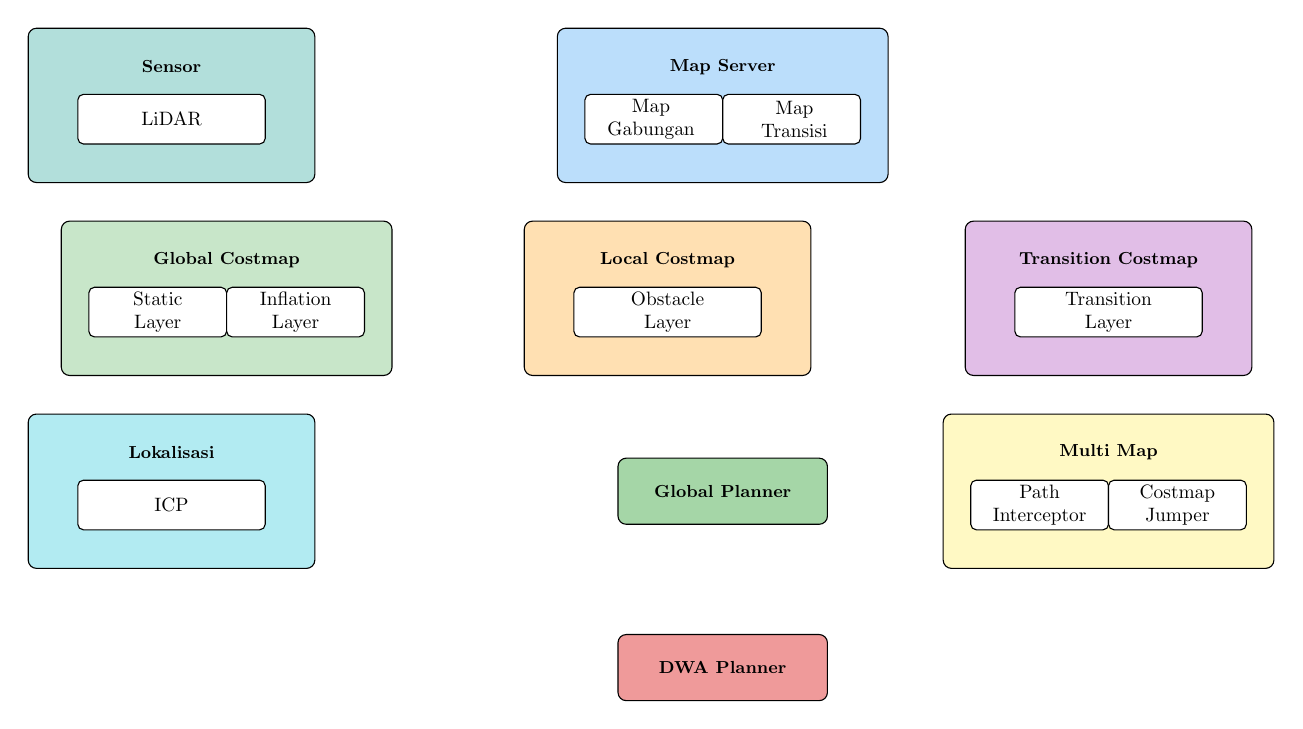
\begin{tikzpicture}[
    scale=0.7, transform shape,
    leaf/.style={
        draw, rounded corners=3pt, minimum width=3.8cm, minimum height=1.2cm,
        align=center, font=\small\bfseries
    },
    subbox/.style={
        draw, rounded corners=2pt, fill=white, minimum width=2.6cm, minimum height=0.9cm,
        align=center, font=\small
    },
    title/.style={font=\small\bfseries, align=center}
]

% ============================
% COLOR DEFINITIONS
% ============================
\definecolor{colSensor}{HTML}{B2DFDB}      % teal light
\definecolor{colMapServer}{HTML}{BBDEFB}   % blue light
\definecolor{colLokalisasi}{HTML}{B2EBF2}  % cyan light
\definecolor{colGlobalCost}{HTML}{C8E6C9}  % green light
\definecolor{colLocalCost}{HTML}{FFE0B2}   % orange light
\definecolor{colTransCost}{HTML}{E1BEE7}   % purple light
\definecolor{colGlobalPlan}{HTML}{A5D6A7}  % green medium
\definecolor{colDWA}{HTML}{EF9A9A}         % red light
\definecolor{colMultiMap}{HTML}{FFF9C4}    % yellow light

% ============================
% ROW 1: Sensor (x=0) & Map Server (x=10)
% ============================

% --- Sensor ---
\draw[fill=colSensor, rounded corners=3pt] (-2.6, -1.4) rectangle (2.6, 1.4);
\node[title] at (0, 0.7) {\textbf{Sensor}};
\draw[fill=white, rounded corners=2pt] (-1.7, -0.7) rectangle (1.7, 0.2);
\node[align=center] at (0, -0.25) {LiDAR};

% --- Map Server ---
\draw[fill=colMapServer, rounded corners=3pt] (7.0, -1.4) rectangle (13.0, 1.4);
\node[title] at (10, 0.7) {\textbf{Map Server}};
\draw[fill=white, rounded corners=2pt] (7.5, -0.7) rectangle (10.0, 0.2);
\node[align=center] at (8.7, -0.25) {Map\\Gabungan};
\draw[fill=white, rounded corners=2pt] (10.0, -0.7) rectangle (12.5, 0.2);
\node[align=center] at (11.3, -0.25) {Map\\Transisi};

% ============================
% ROW 2 (y=-3.5): All Costmaps
% ============================

% --- Global Costmap (x=1) ---
\draw[fill=colGlobalCost, rounded corners=3pt] (-2.0, -4.9) rectangle (4.0, -2.1);
\node[title] at (1, -2.8) {\textbf{Global Costmap}};
\draw[fill=white, rounded corners=2pt] (-1.5, -4.2) rectangle (1.0, -3.3);
\node[align=center] at (-0.25, -3.75) {Static\\Layer};
\draw[fill=white, rounded corners=2pt] (1.0, -4.2) rectangle (3.5, -3.3);
\node[align=center] at (2.25, -3.75) {Inflation\\Layer};

% --- Local Costmap (x=9) ---
\draw[fill=colLocalCost, rounded corners=3pt] (6.4, -4.9) rectangle (11.6, -2.1);
\node[title] at (9, -2.8) {\textbf{Local Costmap}};
\draw[fill=white, rounded corners=2pt] (7.3, -4.2) rectangle (10.7, -3.3);
\node[align=center] at (9, -3.75) {Obstacle\\Layer};

% --- Transition Costmap (x=17) ---
\draw[fill=colTransCost, rounded corners=3pt] (14.4, -4.9) rectangle (19.6, -2.1);
\node[title] at (17, -2.8) {\textbf{Transition Costmap}};
\draw[fill=white, rounded corners=2pt] (15.3, -4.2) rectangle (18.7, -3.3);
\node[align=center] at (17, -3.75) {Transition\\Layer};

% ============================
% ROW 3 (y=-7): Lokalisasi, Global Planner, Multi Map
% ============================

% --- Lokalisasi (x=0) ---
\draw[fill=colLokalisasi, rounded corners=3pt] (-2.6, -8.4) rectangle (2.6, -5.6);
\node[title] at (0, -6.3) {\textbf{Lokalisasi}};
\draw[fill=white, rounded corners=2pt] (-1.7, -7.7) rectangle (1.7, -6.8);
\node[align=center] at (0, -7.25) {ICP};

% --- Global Planner (x=10) ---
\node[leaf, fill=colGlobalPlan] at (10, -7.0) {\textbf{Global Planner}};

% --- Multi Map (x=17) ---
\draw[fill=colMultiMap, rounded corners=3pt] (14.0, -8.4) rectangle (20.0, -5.6);
\node[title] at (17, -6.3) {\textbf{Multi Map}};
\draw[fill=white, rounded corners=2pt] (14.5, -7.7) rectangle (17.0, -6.8);
\node[align=center] at (15.75, -7.25) {Path\\Interceptor};
\draw[fill=white, rounded corners=2pt] (17.0, -7.7) rectangle (19.5, -6.8);
\node[align=center] at (18.25, -7.25) {Costmap\\Jumper};

% ============================
% ROW 4: DWA Planner
% ============================

\node[leaf, fill=colDWA] at (10, -10.2) {\textbf{DWA Planner}};

\end{tikzpicture}
